\appendix

\chapter{Materiales para la recolecci\'on del corpus ZOOM}

\section{Instrucciones para la obtenci\'on del corpus}
\label{corpus-apendice}

En este ap\'endice se muestran los materiales que se usaron para la recolecci\'on del corpus ZOOM. Para ver en detalle informaci\'on del corpus, su recolecci\'on y anotaci\'on vea la Secci\'on \ref{sec:corpus}.

En la Figura \ref{fig-pagPrincipal} se muestra en link que se envi\'o por correo a los participantes que completaron el experimento para la recolecci\'on del corpus ZOOM. En la p\'agina de ven las instrucciones en tres idiomas, la persona ten\'ia que seleccionar el idioma en el que queria completar el experimento. Esta p\'agina conten\'ia las instrucciones en cada uno de los tres idiomas.

\begin{figure}[H]
\begin{center}
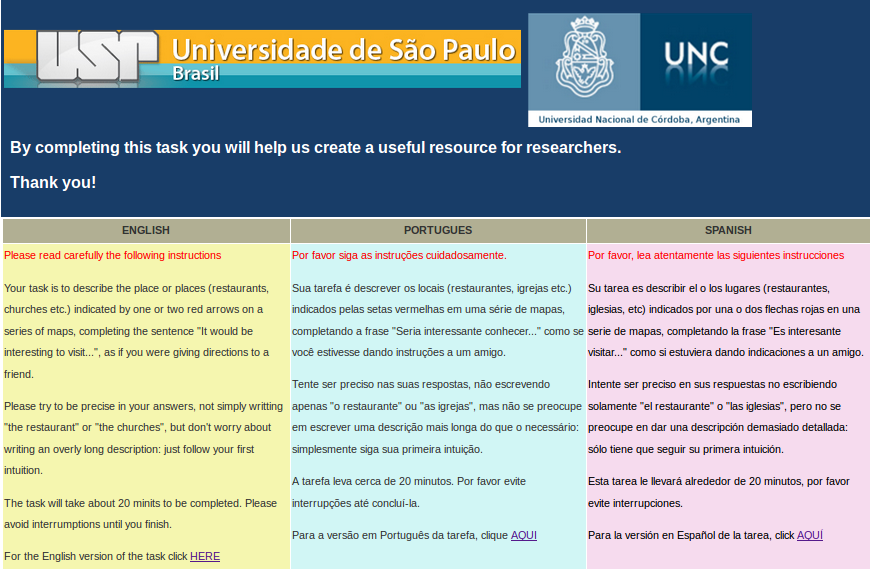
\includegraphics[width=13cm]{images/pagPrincipal.png}\\[0pt]
\caption{Link del experimento.}
\label{fig-pagPrincipal}
\end{center}
\end{figure}

Una vez seleccionado el idioma del experimento, se solicitaba informaci\'on demogr\'afica de los participantes, como se muestra en la Figura \ref{fig-nacionalidadGenero}. Tambi\'en se solicitaba que se acepten los t\'erminos y condiciones los cuales dec\'ian que los datos ingresados ser\'an usados para investigaci\'on.

\begin{figure}[H]
\begin{center}
\frame{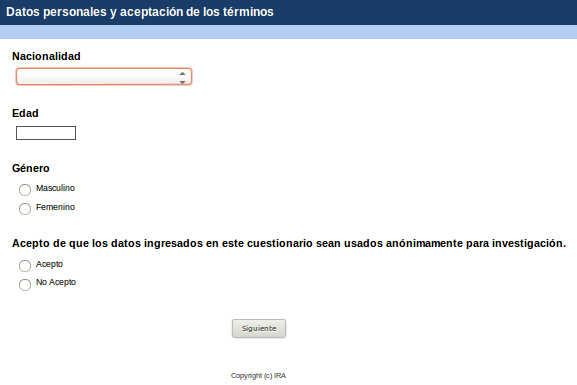
\includegraphics[width=13cm]{images/nacionalidadGenero.png}}
\caption{Datos requeridos.}
\label{fig-nacionalidadGenero}
\end{center}
\end{figure}

En la Figura \ref{fig-interface} se ve una imagen est\'imulo, un mensaje ``Es interesante visitar...'' que es la oraci\'on que el participantente ten\'ia que completar con una expresi\'on referencial del o los objetos apuntados por las flechas. Tambi\'en se ve\'ia una barra indicadora de progreso, y las instrucciones. 

\begin{figure}[H]
\begin{center}
\frame{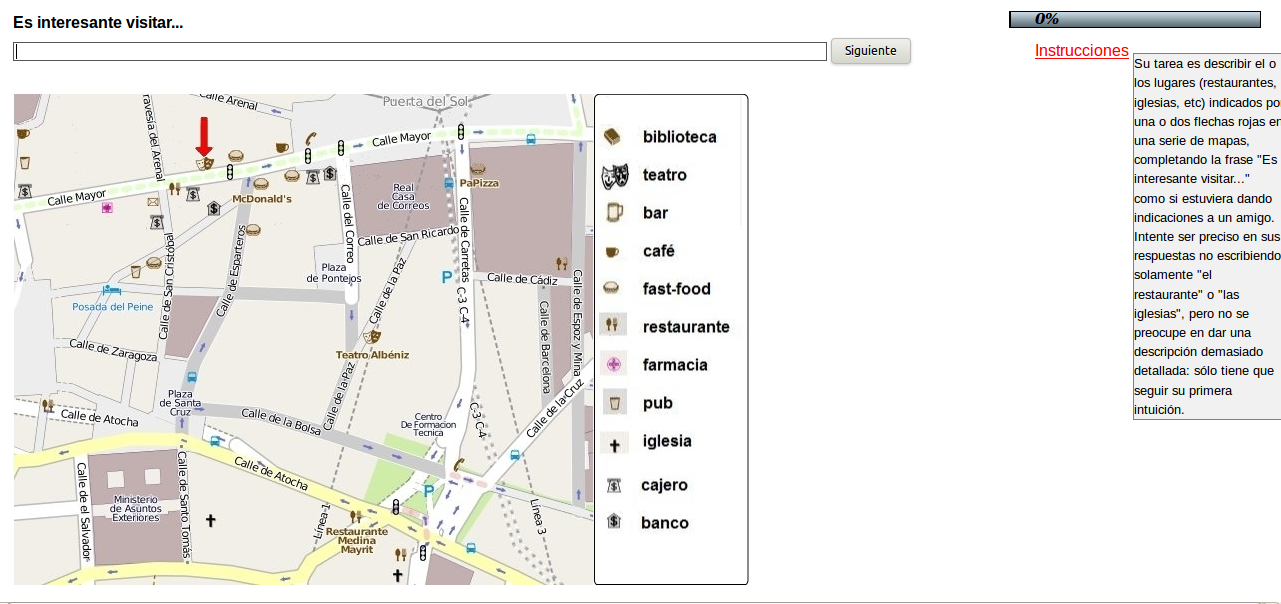
\includegraphics[width=15cm]{images/primerImagen.png}}\\[0pt]
\caption{Interface del experimento.}
\label{fig-interface}
\end{center}
\end{figure}

\section{Im\'agenes est\'imulo del corpus ZOOM}
%\section{}
\label{imagenes-zoom}
%1
Aqu\'i se muestran las im\'agenes que se mostraron a los participantes que completaron la tarea de recolecci\'on del corpus ZOOM para el espa\~nol. El corpus cuenta con im\'agenes con y sin zoom, para targets singulares y plurales. 

\subsection{Est\'imulos singulares}

\begin{figure}[H]
\begin{subfigure}{.48\textwidth}
\centering
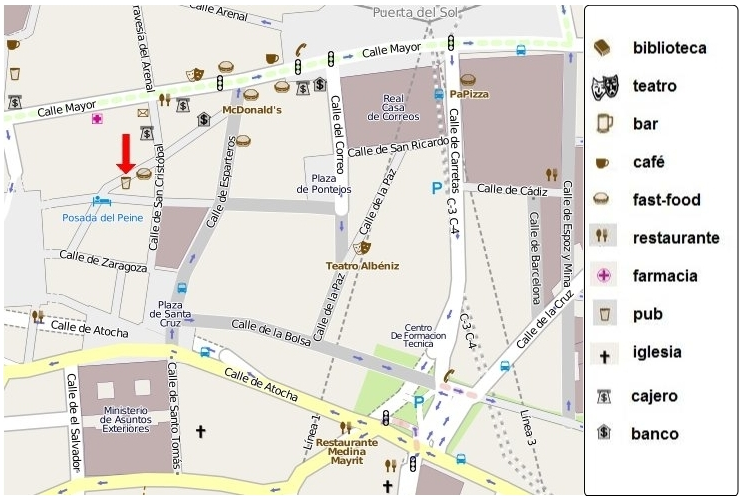
\includegraphics[width=\textwidth]{images/corpus/mapa3.png}
\caption{}
\label{mapa1}
%\vspace*{-0.7cm}
\end{subfigure}
\hspace*{0cm}
\begin{subfigure}{.55\textwidth}
\centering
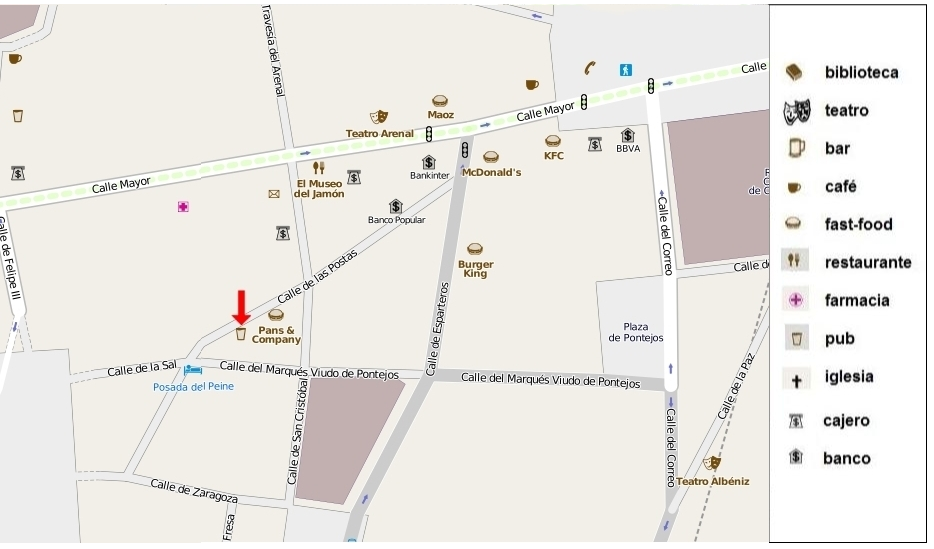
\includegraphics[width=\textwidth]{images/corpus/mapa13.png}
\caption{}
\label{mapa2}
\end{subfigure}
\caption{Imagen del corpus ZOOM. La imagen de la izquierda muestra un target singleton. La imagen de la derecha muestra el mismo target pero con zoom.}
\end{figure}

%2
\begin{figure}[H]
\begin{subfigure}{.48\textwidth}
\centering
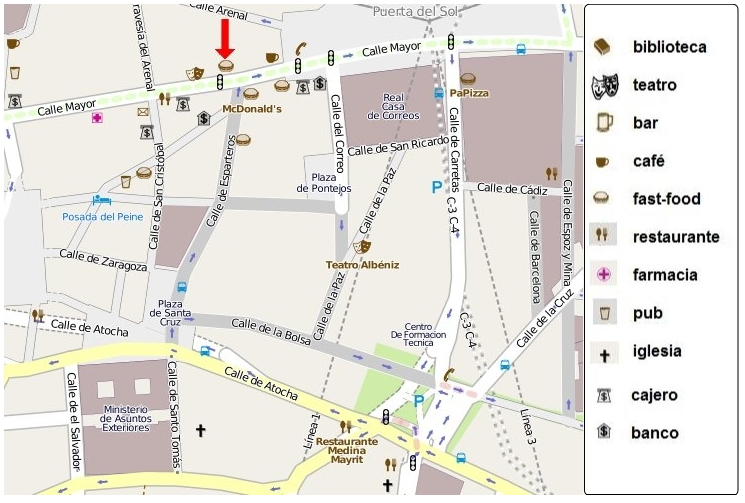
\includegraphics[width=\textwidth]{images/corpus/mapa4.png}
\caption{}
\label{mapa3}
%\vspace*{-0.7cm}
\end{subfigure}
\hspace*{0cm}
\begin{subfigure}{.55\textwidth}
\centering
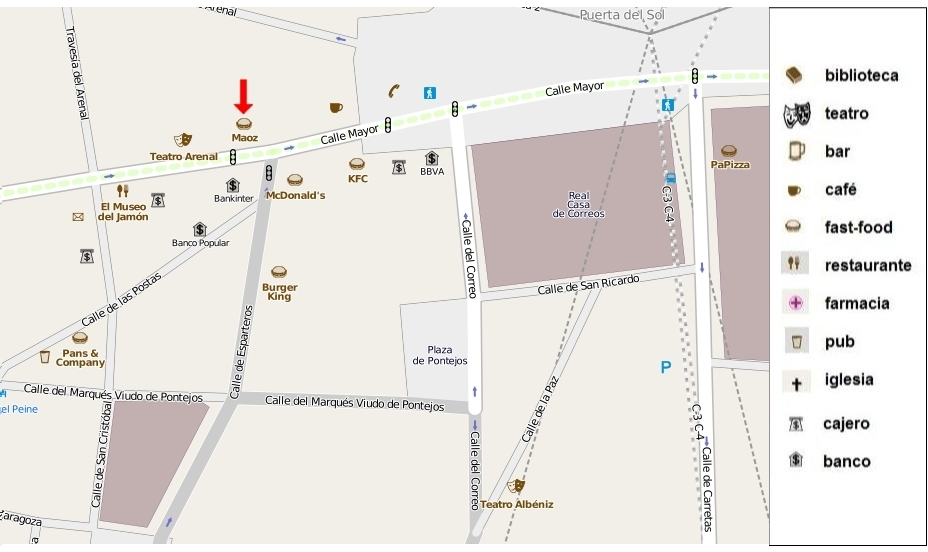
\includegraphics[width=\textwidth]{images/corpus/mapa14.png}
\caption{}
\label{mapa4}
\end{subfigure}
\caption{Imagen del corpus ZOOM. La imagen de la izquierda muestra un target singleton. La imagen de la derecha muestra el mismo target pero con zoom.}
\end{figure}
%3
\begin{figure}[H]
\begin{subfigure}{.48\textwidth}
\centering
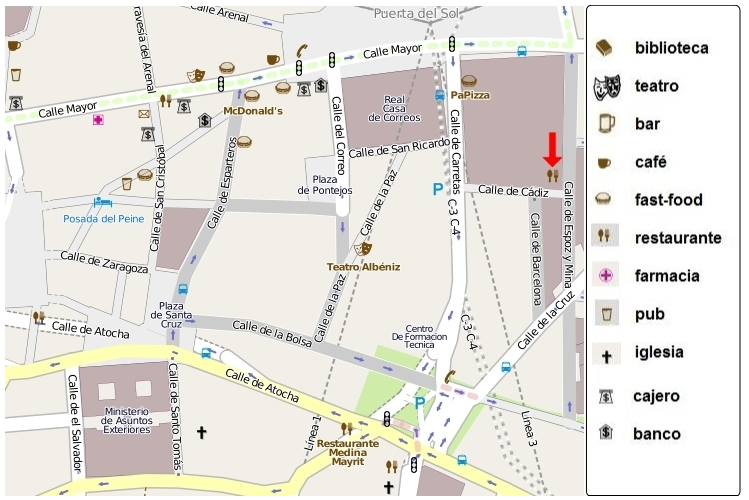
\includegraphics[width=\textwidth]{images/corpus/mapa5.png}
\caption{}
\label{mapa5}
%\vspace*{-0.7cm}
\end{subfigure}
\hspace*{0cm}
\begin{subfigure}{.55\textwidth}
\centering
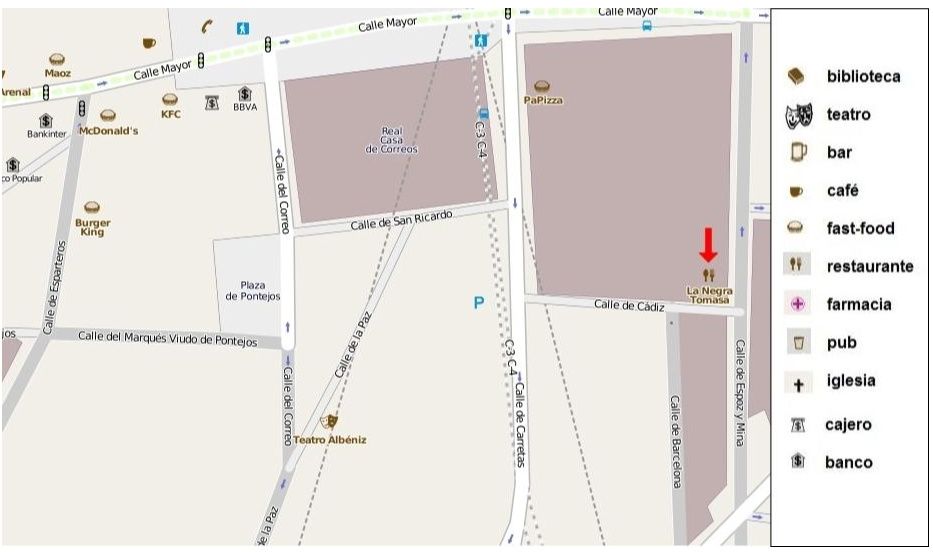
\includegraphics[width=\textwidth]{images/corpus/mapa15.png}
\caption{}
\label{mapa6}
\end{subfigure}
\caption{Imagen del corpus ZOOM. La imagen de la izquierda muestra un target singleton. La imagen de la derecha muestra el mismo target pero con zoom.}
\end{figure}


%4
\begin{figure}[H]
\begin{subfigure}{.48\textwidth}
\centering
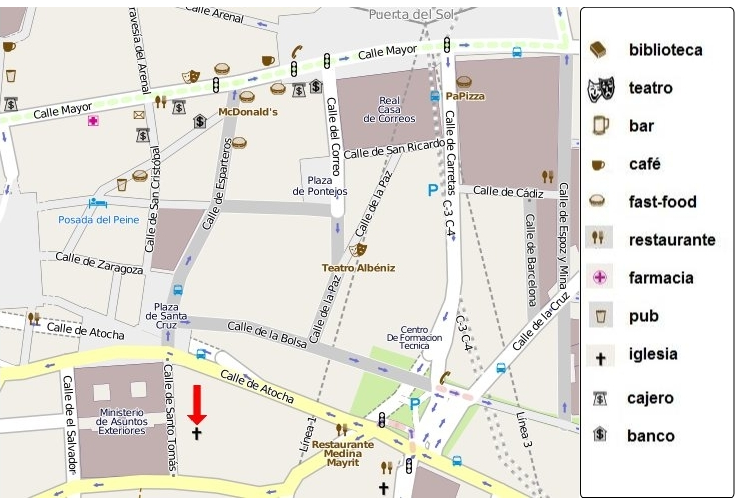
\includegraphics[width=\textwidth]{images/corpus/mapa6.png}
\caption{}
\label{mapa15}
%\vspace*{-0.7cm}
\end{subfigure}
\hspace*{0cm}
\begin{subfigure}{.55\textwidth}
\centering
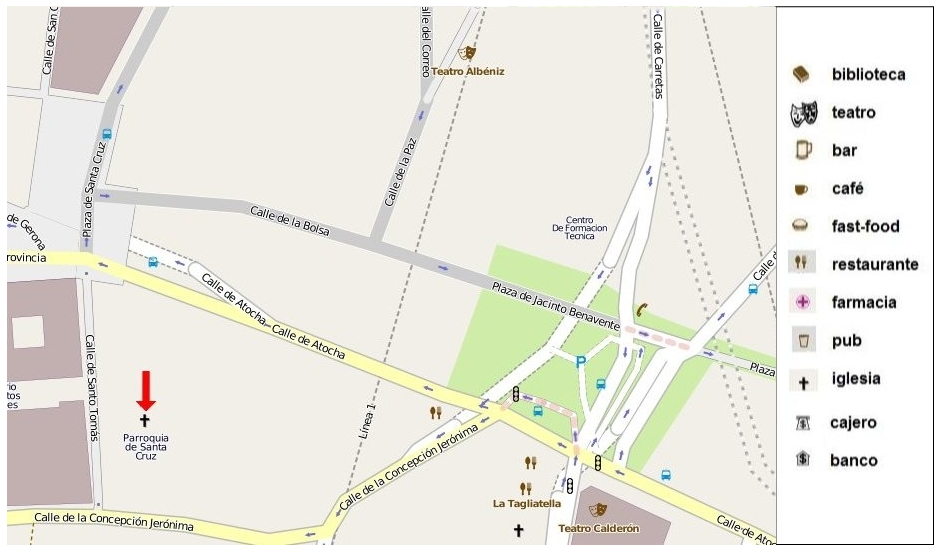
\includegraphics[width=\textwidth]{images/corpus/mapa16.png}
\caption{}
\label{mapa16}
\end{subfigure}
\caption{Imagen del corpus ZOOM. La imagen de la izquierda muestra un target singleton. La imagen de la derecha muestra el mismo target pero con zoom.}
\end{figure}

%5
\begin{figure}[H]
\begin{subfigure}{.48\textwidth}
\centering
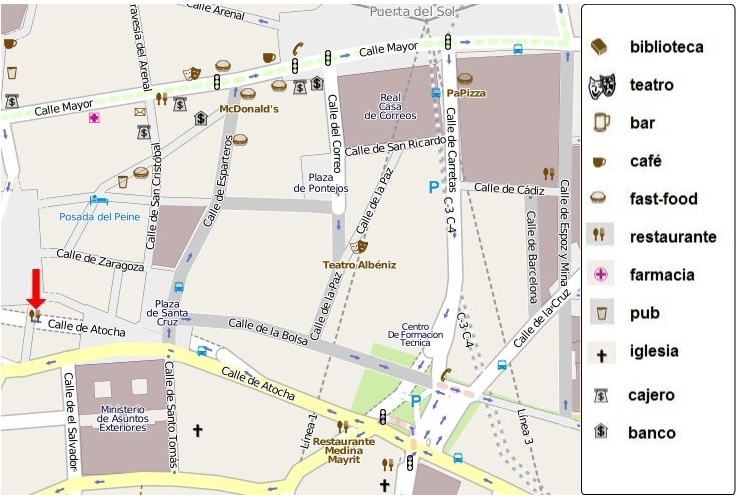
\includegraphics[width=\textwidth]{images/corpus/mapa7.png}
\caption{}
\label{mapa9}
%\vspace*{-0.7cm}
\end{subfigure}
\hspace*{0cm}
\begin{subfigure}{.55\textwidth}
\centering
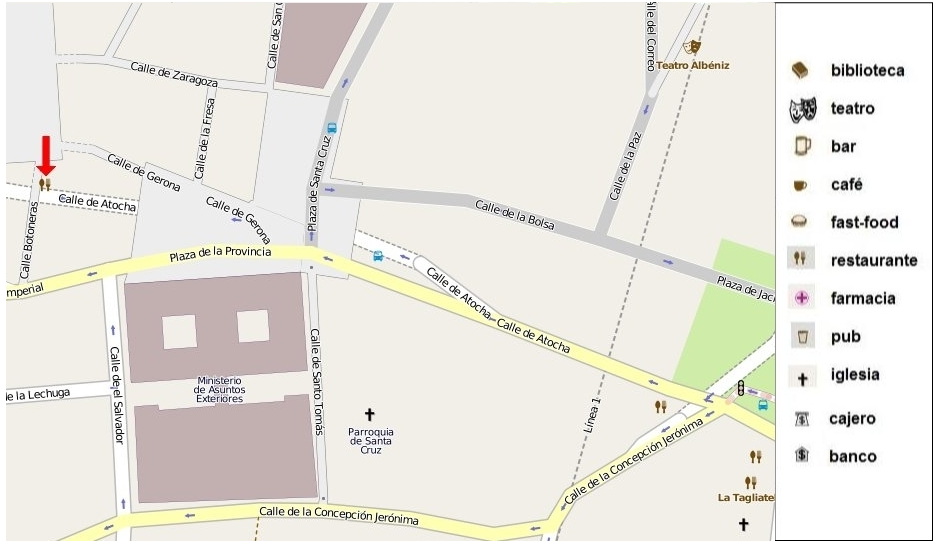
\includegraphics[width=\textwidth]{images/corpus/mapa17.png}
\caption{}
\label{mapa10}
\end{subfigure}
\caption{Imagen del corpus ZOOM. La imagen de la izquierda muestra un target singleton. La imagen de la derecha muestra el mismo target pero con zoom.}
\end{figure}

%6
\begin{figure}
\begin{subfigure}{.48\textwidth}
\centering
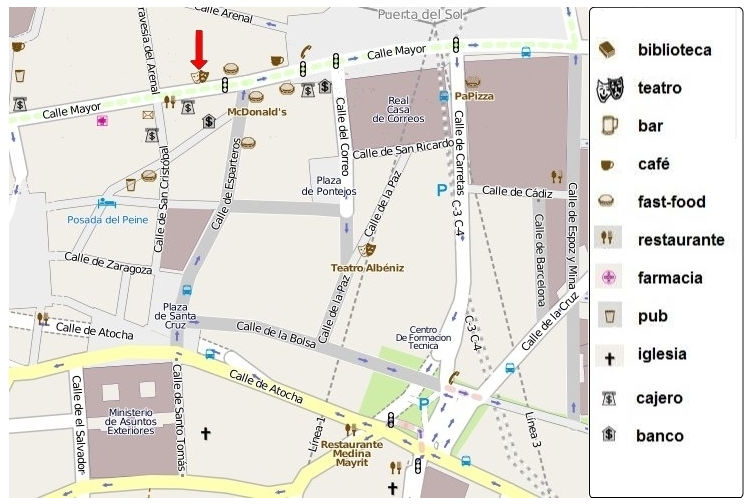
\includegraphics[width=\textwidth]{images/corpus/mapa1.png}
\caption{}
\label{mapa13}
%\vspace*{-0.7cm}
\end{subfigure}
\hspace*{0cm}
\begin{subfigure}{.55\textwidth}
\centering
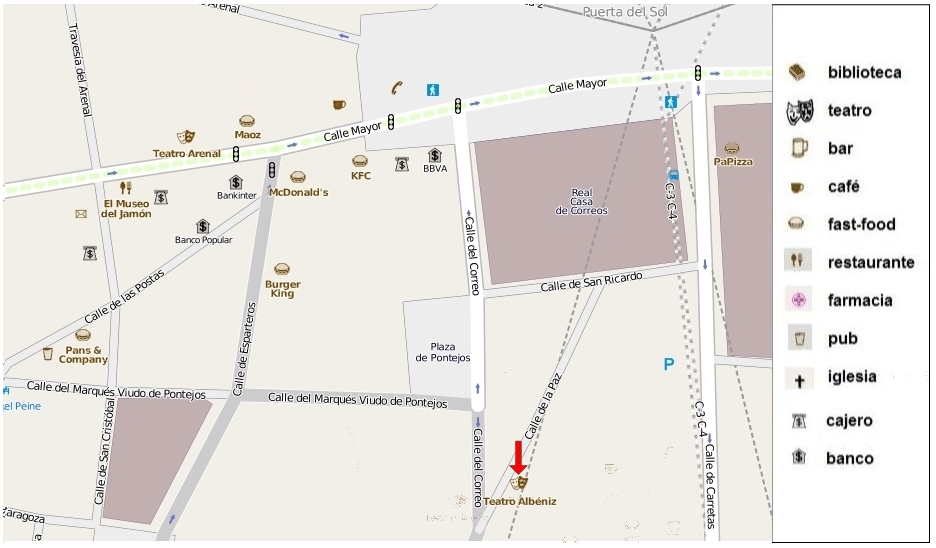
\includegraphics[width=\textwidth]{images/corpus/mapa2.png}
\caption{}
\label{mapa14}
\end{subfigure}
\caption{Imagen del corpus ZOOM. La imagen de la izquierda muestra un target singleton. La imagen de la derecha muestra el mismo target pero con zoom.}
\end{figure}
%7
\subsection{Est\'imulos plurales}
\begin{figure}
\begin{subfigure}{.48\textwidth}
\centering
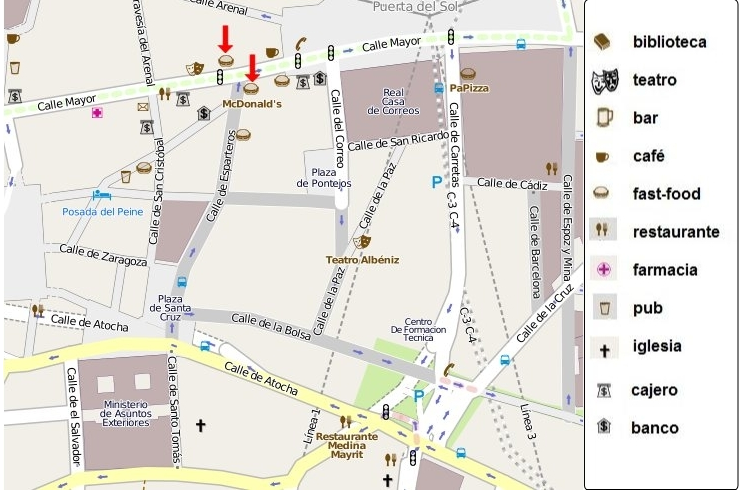
\includegraphics[width=\textwidth]{images/corpus/mapa8.png}
\caption{}
\label{mapa7}
%\vspace*{-0.7cm}
\end{subfigure}
\hspace*{0cm}
\begin{subfigure}{.55\textwidth}
\centering
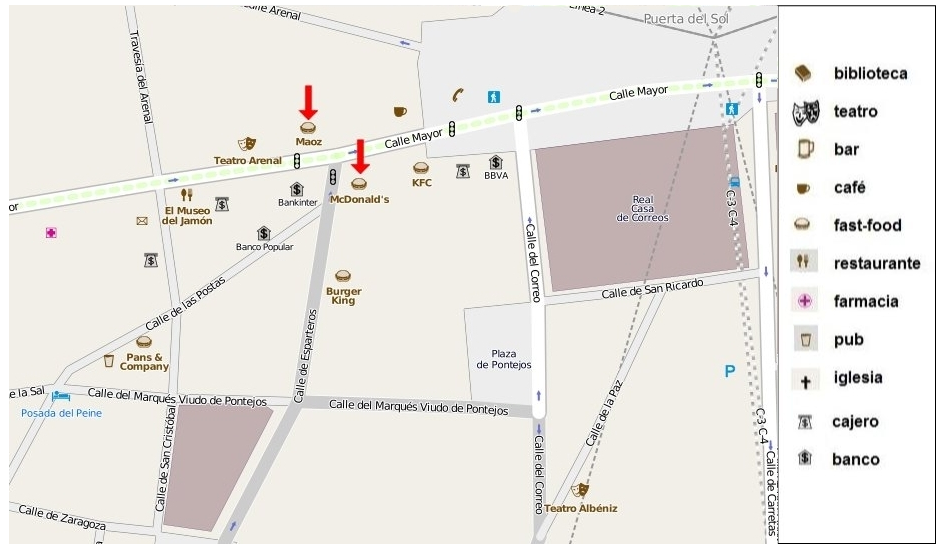
\includegraphics[width=\textwidth]{images/corpus/mapa18.png}
\caption{}
\label{mapa8}
\end{subfigure}
\caption{Imagen del corpus ZOOM. La imagen de la izquierda muestra target plural. La imagen de la derecha muestra el mismo target pero con zoom.}
\end{figure}

%8

\begin{figure}
\begin{subfigure}{.48\textwidth}
\centering
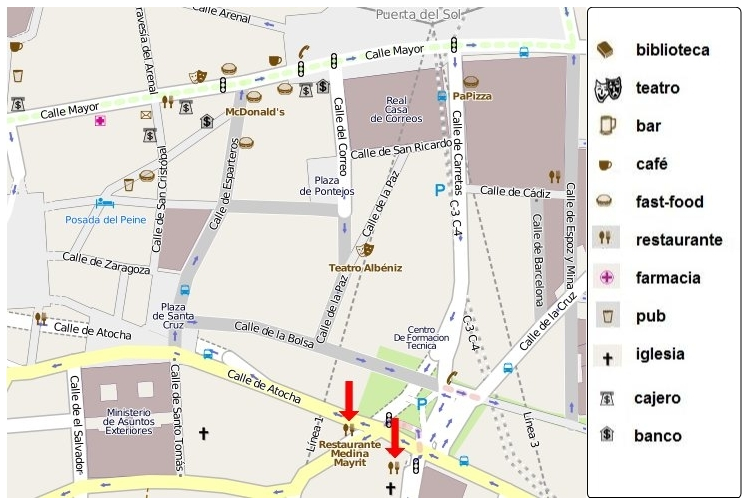
\includegraphics[width=\textwidth]{images/corpus/mapa10.png}
\caption{}
\label{mapa17}
%\vspace*{-0.7cm}
\end{subfigure}
\hspace*{0cm}
\begin{subfigure}{.55\textwidth}
\centering
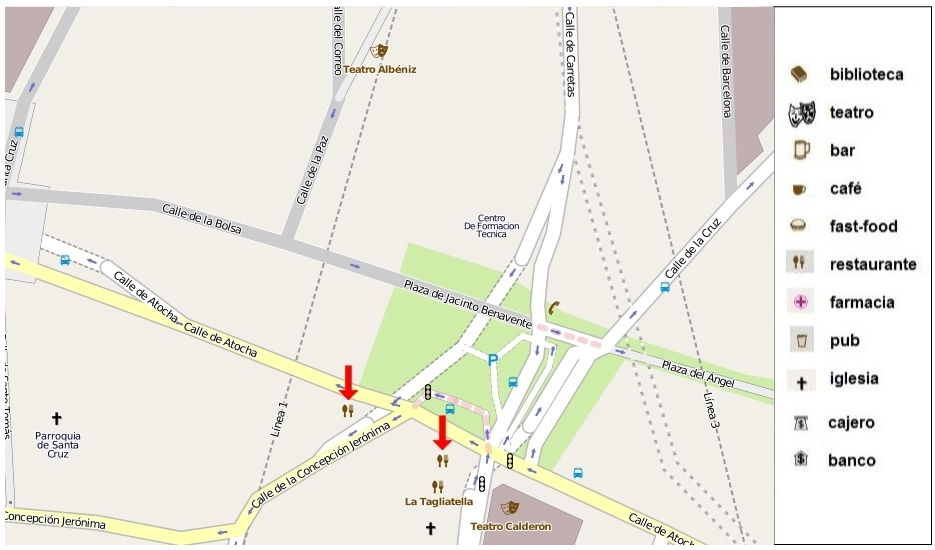
\includegraphics[width=\textwidth]{images/corpus/mapa20.png}
\caption{}
\label{mapa18}
\end{subfigure}
\caption{Imagen del corpus ZOOM. La imagen de la izquierda muestra target plural. La imagen de la derecha muestra el mismo target pero con zoom.}

\end{figure}
%9

\begin{figure}
\begin{subfigure}{.48\textwidth}
\centering
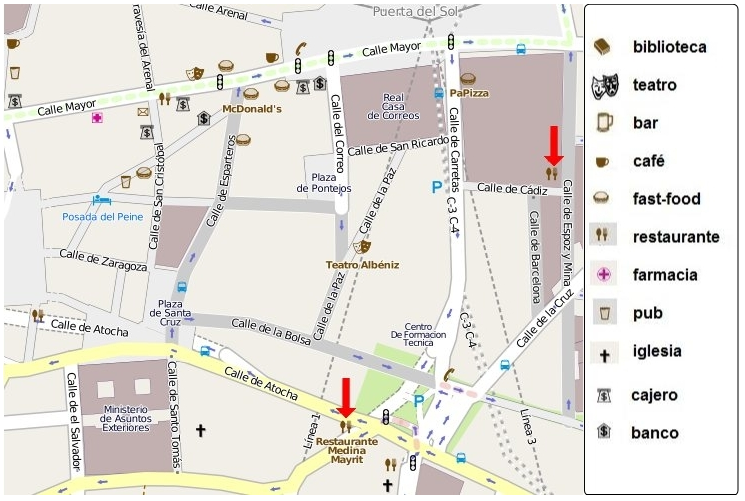
\includegraphics[width=\textwidth]{images/corpus/mapa9.png}
\caption{}
\label{mapa19}
%\vspace*{-0.7cm}
\end{subfigure}
\hspace*{0cm}
\begin{subfigure}{.55\textwidth}
\centering
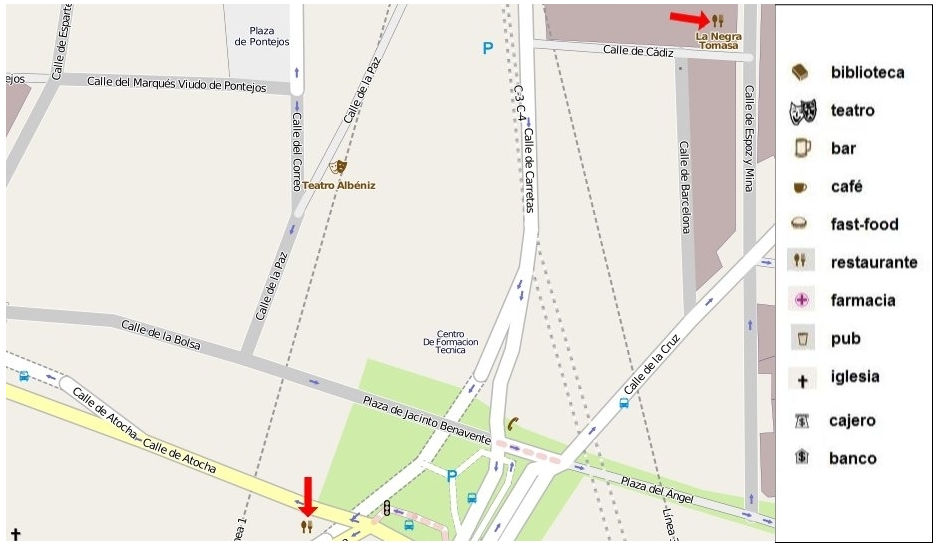
\includegraphics[width=\textwidth]{images/corpus/mapa19.png}\\[0pt]
\caption{}
\label{mapa20}
\end{subfigure}
\caption{Imagen del corpus ZOOM. La imagen de la izquierda muestra target plural. La imagen de la derecha muestra el mismo target pero con zoom.}

\end{figure}

\begin{figure}
\begin{subfigure}{.55\textwidth}
\centering
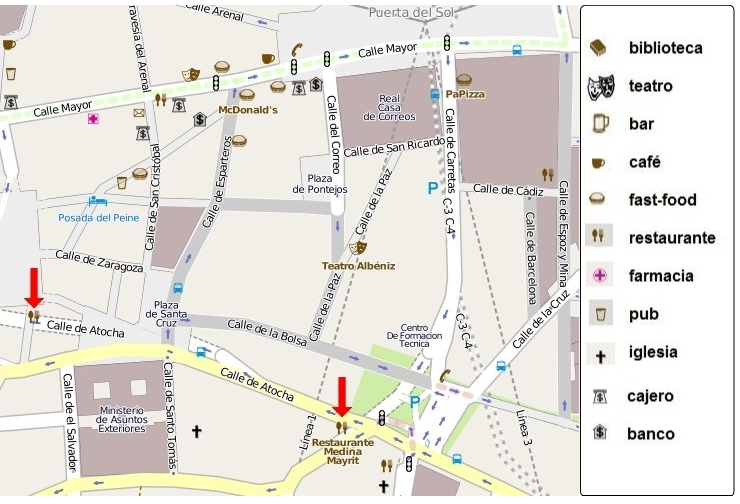
\includegraphics[width=\textwidth]{images/corpus/mapa11.png}
\caption{}
\label{mapa11}
%\vspace*{-0.7cm}
\end{subfigure}
\hspace*{0cm}
\begin{subfigure}{.55\textwidth}
\centering
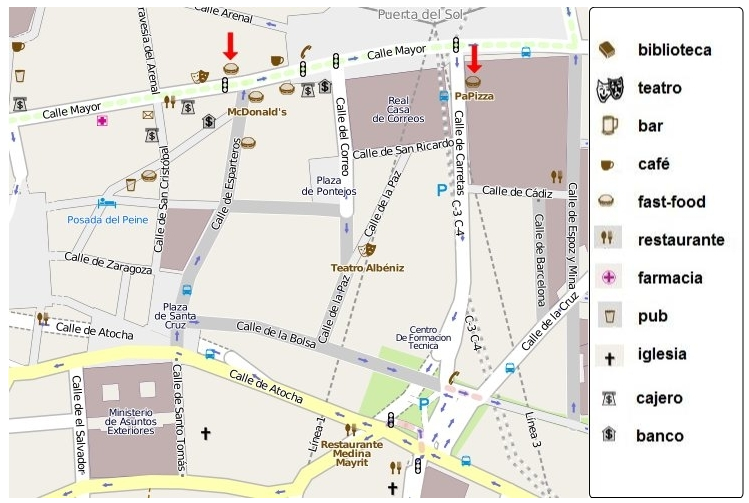
\includegraphics[width=\textwidth]{images/corpus/mapa12.png}
\caption{}
\label{mapa12}
\end{subfigure}
\caption{Imagen del corpus ZOOM. La imagen de la izquierda muestra target plural 2 restaurantes. La imagen de la derecha muestra 2 fast-foods como targets.}

\end{figure}

\chapter{Expresiones referenciales generadas por nuestro algoritmo}

\section{ERs dadas por el algoritmo para corpus ZOOM}
%\section{}
\label{er-mapa-zoom}

%\begin{table}[h]
%\begin{center}
%\begin{tabular}{|l|l|c|}
%\hline
%&F\'ormula			      &  \# \\ \hline \hline

%1 & $\exists \nChurchSin \land \exists \nIn .(\exists \nCalleSantoTomas) $&234 \\ \hline

%2 & $\exists \nFront . (\exists \nMinAsExt)$&202 \\ \hline

%3& $\exists \nChurch \land \exists \nIn .(\exists \nCalleAtocha)$&87 \\ \hline

%4& $\exists \nNear .(\exists \nMinAsExt)$&79 \\ \hline

%5& $\exists \nFront .(\exists \nFront .(\exists \nChurch)) \land \exists \nIn .(\exists \nCalleSantoTomas)$&74 \\ \hline

%6& $\exists \nChurch \land \exists \nFront .(\exists \nMinAsExt)$&71 \\ \hline

%7& $\exists \nChurch \land \exists \nFront .(\exists \nMinAsExt \land \exists \nIn)$&65 \\ \hline

%8& $\exists \nFront .(\exists \nIn (\exists \nCalleSantoTomas)) \land \exists \nChurch \land \exists \nIn$&53 \\ \hline

%9& $\exists \nFront .(\exists \nMinAsExt \land \exists \nIn )$&21 \\ \hline

%10&$\exists \nNear .(\exists \nMinAsExt \land \exists \nIn )$&15 \\

%\hline
%\end{tabular}

%\caption{Las 10 f\'ormulas m\'as frecuentes dadas por el algoritmo para el modelo de la Figura \protect\ref{modelo-mapa-zoom}.}\label{formulas-mapa-zoom}
%\end{center}
%\end{table}




%\footnotesize{
%\hspace*{0.6cm}

Las f\'ormulas mostradas en la Tabla \ref{formulas-mapa-zoom-ap}, fueron generadas por el algoritmo en el caso de estudio presentado en la Secci\'on \ref{sec:sinzoom}. Ejecutando el algoritmo 1000 veces.

\begin{table}[H]
\begin{center}
\begin{tabular}{|l|l|c|}
\hline
&F\'ormula			      &  \# \\ \hline \hline

1&$\exists \nChurch.(T) \land \exists \nIn .(\exists \nCalleSantoTomas))$ &234 \\ \hline

2&$\exists \nFront . (\exists \nMinAsExt)$ &202 \\ \hline

3&$\exists \nChurch.(T) \land \exists \nIn .(\exists \nCalleAtocha)$ &87\\ \hline

4&$\exists \nNear .(\exists \nMinAsExt .(T))$ &79\\ \hline

5&$\exists \nFront.(\exists \nFront.(\exists \nChurch.(T))) \land \exists \nIn .(\exists \nCalleSantoTomas))$ &74\\ \hline

6&$\exists \nChurch.(T) \land \exists\nFront . (\exists \nMinAsExt))$ &71\\ \hline

7&$\exists \nChurch.(T) \land \exists\nFront . (\exists \nMinAsExt) \land \exists \nIn .(T))$ &65\\ \hline

8&$\exists \nFront.(\exists \nIn .(\exists \nCalleSantoTomas))) \land \exists \nChurch.(T) \land \exists \nIn .(T)$ &53\\ \hline

9&$\exists \nFront . (\exists \nMinAsExt) \land \exists \nIn .(T))$ &21\\ \hline

10&$\exists \nNear .(\exists \nMinAsExt .(T) \land \exists \nIn .(T))$ &15\\ \hline

11&$\exists  \nNear.(\exists \nIn .(\exists \nCalleSantoTomas))) \land \exists \nChurch.(T)$ &13\\ \hline

12&$\exists  \nNear.(\exists \nFront.(\exists \nChurch.(T))) \land \exists \nIn .(\exists \nCalleAtocha)$ &11\\ \hline

13&$\exists \nFront.(\exists \nIn .(\exists \nCalleSantoTomas))) \land \exists \nChurch.(T)$ &11\\ \hline

14&$\exists \nChurch.(T) \land \exists \nIn .(\exists \nCalleAtocha) \land \exists \nFront.(\exists \nFront.(\exists \nChurch.(T)))$ &10\\ \hline

15&$\exists  \nNear.(\exists \nNear.(\exists \nChurch.(T))) \land \exists \nIn .(\exists \nCalleSantoTomas))$ &8\\ \hline

16&$\exists  \nNear.(\exists \nIn .(\exists \nCalleSantoTomas))) \land \exists \nChurch.(T) \land \exists \nIn .(T)$ &6\\ \hline

17&$\exists \nChurch.(T) \land \exists \nNear .(\exists \nMinAsExt .(T) \land \exists \nIn .(T))$ &6\\ \hline

18&$\exists  \nNear.(\exists \nNear.(\exists \nChurch.(T) \land \exists \nIn .(T))) \land \exists \nIn .(\exists \nCalleSantoTomas))$ &5\\ \hline

19&$\exists \nFront.(\exists \nFront.(\exists \nChurch.(T) \land \exists \nIn .(T))) \land \exists \nIn .(\exists \nCalleSantoTomas))$ &5\\ \hline

20&$\exists  \nIn .(\exists \nCalleSantoTomas)) \land \exists \nChurch.(T)$ &4\\ \hline

21&$\exists \nChurch.(T) \land \exists \nNear .(\exists \nMinAsExt .(T))$ &4\\ \hline

22&$\exists  \nNear.(\exists \nFront.(\exists \nChurch.(T))) \land \exists \nIn .(\exists \nCalleSantoTomas))$ &4\\ \hline

23&$\exists \nFront.(\exists \nNear.(\exists \nChurch.(T))) \land \exists \nIn .(\exists \nCalleSantoTomas))$ &3\\ \hline

24&$\exists \nChurch.(T) \land \exists \nNear.(\exists \nNear.(\exists \nChurch.(T))) \land \exists \nIn .(\exists \nCalleAtocha)$ &2\\ \hline

25&$\exists  \nNear.(\exists \nFront.(\exists \nChurch.(T) \land \exists \nIn .(T))) \land \exists \nIn .(\exists \nCalleAtocha)$ &2\\ \hline

26&$\exists \nChurch.(T) \land \exists \nIn .(\exists \nCalleAtocha) \land \exists \nNear.(\exists \nNear.(\exists \nChurch.(T)))$ &2\\ \hline

27&$\exists \nFront.(\exists \nIn .(\exists \nCalleSantoTomas))) \land \exists \nNear.(\exists \nNear.(\exists \nChurch.(T)))$ &1\\ \hline

28&$\exists \nFront . (\exists \nMinAsExt) \land \exists \nIn .(\exists \nCalleAtocha))$ &1\\ \hline

29&$\exists  \nIn .(\exists \nCalleAtocha) \land \exists \nChurch.(T)$ &1\\ \hline

\end{tabular}

\caption{F\'ormulas dadas por el algoritmo para el modelo de la Figura \protect\ref{modelo-mapa-zoom}.}\label{formulas-mapa-zoom-ap}
\end{center}
\end{table}


En la Tabla \ref{formulas-mapa-zoom2x-apendice} se muestran las f\'ormulas generadas por el algoritmo para el caso de estudio mostrado en la Secci\'on \ref{sec:conzoom}, ejecutando el algoritmo 1000 veces.

\begin{table}[H]
\begin{center}
\begin{tabular}{|l|l|c|}
\hline
&F\'ormula                           &  \# \\ \hline \hline
1& $\exists \nParroquiaDeSantaCruz$& 570\\ \hline

2& $\exists \nParroquiaDeSantaCruz. \exists \nIn(T)$& 174\\ \hline
3& $\exists \nParroquiaDeSantaCruz. \exists \nIn(\exists \nCalleSantoTomas)$& 72\\ \hline
4& $\exists \nParroquiaDeSantaCruz. \land \exists.\nCerca(T)$& 57\\ \hline

5& $\exists \nChurch \land \exists \nParroquiaDeSantaCruz$& 48\\ \hline
6& $\exists \nChurch \land \exists \nParroquiaDeSantaCruz. \exists \nIn(T)$& 17\\ \hline
7& $\exists \nParroquiaDeSantaCruz \land \exists. \nIn(\exists \nCalleConJer)$& 13\\ \hline
8& $\exists \nChurch \land \land \exists. \nIn(\exists \nCalleConJer) $&10\\ \hline

9& $\exists \nIn(\exists \nCalleSantoTomas) \land \exists \nChurch$&9\\ \hline

10& $\exists \nChurch \land \exists \nIn(\exists \nCalleSantoTomas))$&7\\ \hline

\end{tabular}

\caption{F\'ormulas dadas por el algoritmo para el modelo de la Figura \protect\ref{modelo-mapa-zoom2x}.}\label{formulas-mapa-zoom2x-apendice}
\end{center}
\end{table}

En la Tabla \ref{formulas-mapa-zoom2-apendice} se muestran las f\'ormulas dadas por el algoritmo en 1000 ejecuciones para la Figura \ref{mapa-zoom-plural}, mostrado en la Secci\'on \ref{sec:plural}, ejecutando el algoritmo 1000 veces. 

\label{formulas-plurales}
\begin{table}[H]
\begin{center}
\begin{tabular}{|l|l|c|}
\hline
&F\'ormula			      &  \# \\ \hline \hline

1&$rest_3 = \exists \nMedinaMayrit$ &303\\
 &$rest_4 = \exists \nNear.(\exists \nMedinaMayrit)$& \\ \hline

2&$rest_3 = \exists \nMedinaMayrit$ & 285\\  
 &$rest_4 =  \exists \nNear. (\exists \nNear.(\exists \nMedinaMayrit)) \land \exists \nNear.(\exists \nMedinaMayrit)$& \\ \hline

3&$rest_3 =\exists \nMedinaMayrit \land \exists \nIn.(T)$ & 105\\ 
 &$rest_4 =\exists \nNear.(\exists \nMedinaMayrit \land \exists \nIn.(T))$& \\ \hline

4&$rest_3 =\exists \nMedinaMayrit \land \exists \nIn.(\exists \nCalleAtocha)$ &83 \\ 
 &$rest_4 =\exists \nNear.(\exists \nMedinaMayrit  \land \exists \nIn.(\exists \nCalleAtocha))$& \\ \hline

5&$rest_3 =\exists \nMedinaMayrit  \land \exists \nIn.(\exists \nCalleAtocha)$&77 \\ 
 &$\land \exists \nNear.(\exists \nNear.(\exists \nMedinaMayrit))$& \\
&$rest_4 = \exists \nNear.(\exists \nMedinaMayrit)$& \\ \hline

6&$rest_3 =\exists \nNear.(\exists \nIn.(\exists \nCalleDeLaCruz))  \land \exists \nIn.(\exists \nCalleDeCarretas) \land $ & 20\\
&$\exists \nIn.(\exists \nCalleDeLaCruz)  \land \exists \nNear.(\exists \nIn.(\exists \nCalleDeCarretas))$& \\ \hline

7&$rest_3 =\exists \nMedinaMayrit  $&13 \\ 
&$\land \exists \nNear.(\exists \nIn.(\exists \nCalleDeLaCruz))  \land \exists \nIn.(\exists \nCalleAtocha)$ & \\
&$rest_4 = \exists \nNear.(\exists \nMedinaMayrit)$&\\ \hline

8&$rest_3 =\exists \nIn.(\exists \nCalleDeCarretas)  \land \exists \nNear.(\exists \nNear.$&9\\
&$(\exists \nNear.(\exists \nNear.(\exists$ &\\
&$\nNear.(\exists \nIn.(\exists \nCalleDeCarretas)))))) $&\\
&$rest_4 = \exists \nNear.(\exists \nIn.(\exists \nCalleDeCarretas)  $ & \\
&$\land \exists \nNear.(\exists \nNear.(\exists \nNear.(\exists \nNear.(\exists \nNear.$&\\
&$(\exists \nIn.(\exists \nCalleDeCarretas)))))))$&\\ \hline

9&$rest_3 =\exists \nMedinaMayrit \land \exists \nIn.(\exists \nCalleAtocha)$ & 9\\
&$rest_4 = \exists \nNear.(\exists \nIn.(\exists \nCalleAtocha) $ & \\
&$ \land \exists \nNear.(\exists \nNear.(\exists \nChurch.(T)  \land \exists \nNear.(\exists \nIn.(\exists \nCalleAtocha)  $ & \\
&$\land \exists \nNear.(\exists \nNear.(\exists \nChurch.(T)  \land \exists \nIn.(T)))))))$&\\ \hline

10&$rest_3 = \exists \nNear.(\exists \nIn.(\exists \nCalleAtocha)  \land \exists \nNear.(\exists \nNear.(\exists \nIn.(\exists \nCalleAtocha) $ & 9\\
&$ \land \exists \nNear.(\exists \nNear.(\exists \nIn.(\exists \nCalleDeCarretas))))))  \land \exists \nIn.(\exists \nCalleDeCarretas)  $ & \\
&$rest_4 = \exists \nNear.(\exists \nNear.(\exists \nIn.(\exists \nCalleAtocha)  \land \exists \nNear.(\exists \nNear.$ & \\
&$(\exists \nIn.(\exists \nCalleAtocha)  \land \exists \nNear.(\exists \nNear.(\exists \nIn.(\exists \nCalleDeCarretas)))))) $ & \\
&$ \land \exists \nIn.(\exists \nCalleDeCarretas))$&\\ \hline

\end{tabular}

\caption{Las 10 f\'ormulas m\'as frecuentes dadas por el algoritmo para el modelo de la Figura \protect\ref{modelo-mapa-zoom}. Tomando como target 2 restaurantes.}\label{formulas-mapa-zoom2-apendice}
\end{center}
\end{table}

\section{Generaci\'on sobre el corpus GRE3D7}

\subsection{Ejemplos de f\'ormulas}
\label{formulas-gre3d7}

En la Secci\'on \ref{sec:ejemplo_ejecucion} se mostr\'o un ejemplo de ejecuci\'on del algoritmo para la Figura \ref{GRE3D7-stimulus-22-apendice}, aqu\'i mostramos todas las f\'ormulas que di\'o el algoritmo para el target se\~nalado por la flecha, en 10000 ejecuciones.

\begin{figure}[h]
%\begin{subfigure}{0.5\linewidth}
\centering
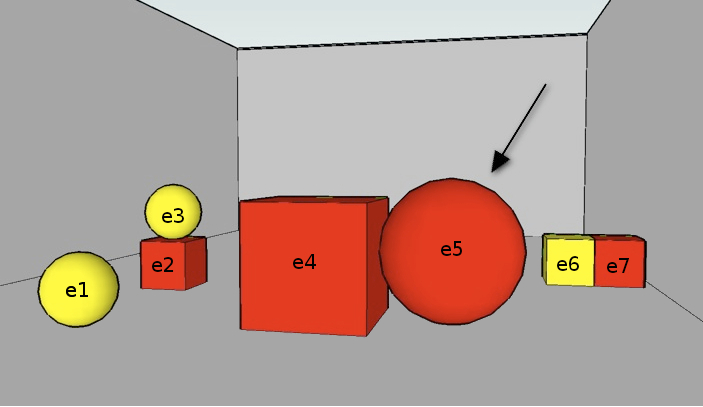
\includegraphics[width=\textwidth]{images/22.jpg}
%\vspace*{1cm}
\caption{Escena del corpus GRE3D7.}
\label{GRE3D7-stimulus-22-apendice}
\end{figure}


\begin{table}[h]
\begin{center}
\begin{tabular}{|l|l|c|}
\hline
&F\'ormula			      &  \# \\ \hline \hline

1&$\exists \nBall \land \exists \nLarge \land \exists \aRed$		&6003 \\ \hline
2&$\exists \nBall \land \exists \aRed$		&3672 \\ \hline
3&$\exists \nBall \land \exists \nLarge$		&53 \\ \hline
4&$\exists \nBall \land \exists \aRed \land \exists \nRightof$	&	248 \\ \hline
5&$\exists \nBall \land \exists \nRightof$		&15 \\ \hline
6&$\exists \nBall \land \exists \nRightof(\exists \nCube)$	&	7 \\ \hline
7&$\exists \nBall \land \exists \nRightof(\exists \nCube \land \exists \nLarge)$&		1 \\ \hline
8&$\exists \nBall \land \exists \nRightof(\exists \nCube \land \exists \aRed)$		&1 \\ \hline

\end{tabular}

\caption{F\'ormulas dadas por el algoritmo para el modelo de la Figura \protect\ref{fig4-9}.}\label{formulas-mapa-gre3d7-apendice}
\end{center}
\end{table}

\subsection{Im\'agenes verde-azules del corpus}
\label{imagenesGRE3D7-apendice}
En la Figura \ref{verde-azul} se muestran las escenas mostradas a los participantes del corpus \textit{GRE3D7} introducido en la Secci\'on \ref{sec:corpusGRE}, esta parte incluye s\'olo las escenas verde y azules. El corpus contiene otra parte similar con colores rojo y amarillo.

\begin{figure}[h]
\centering
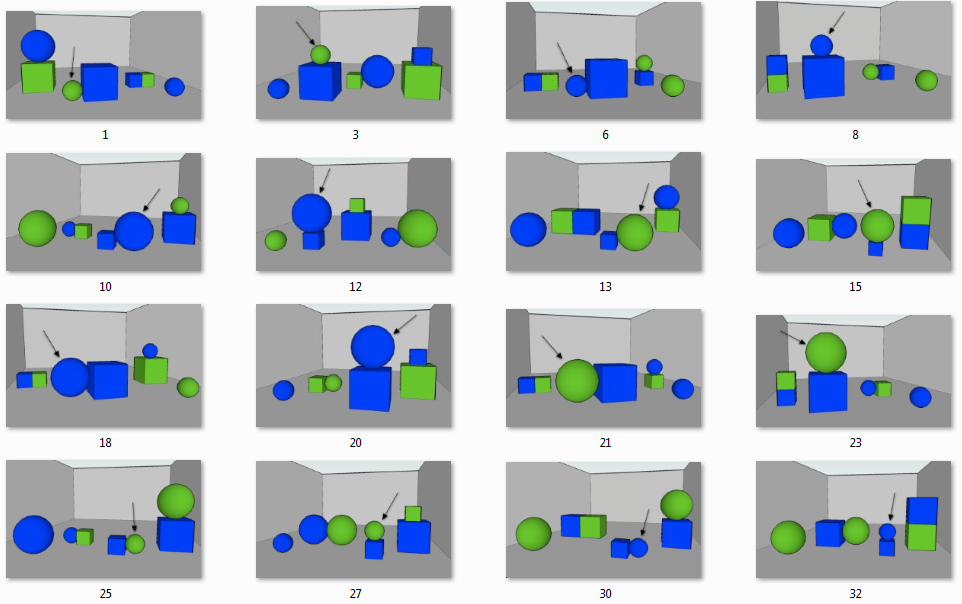
\includegraphics[width=1\textwidth]{images/corpusVerdeAzul.png}
%\vspace{-0.5}
\caption{Im\'agenes del \textit{GRE3D7} parte azul y verde.}
\label{verde-azul}
\end{figure}




%\chapter{Archivo xml del TUNA corpus}
%\section{Archivo}
%\label{archivos-xml-tuna}
%
%Este es el texto del archivo s57t4.xml del TUNA corpus.
%\begin{verbatim}
%<TRIAL CONDITION="-LOC" ID="s57t4">
  %<DOMAIN>
    %<ENTITY ID="121" IMAGE="fanLeftBlueSmall.gif" TYPE="target">
      %<ATTRIBUTE NAME="colour" TYPE="literal" VALUE="blue" />
      %<ATTRIBUTE NAME="orientation" TYPE="literal" VALUE="left" />
      %<ATTRIBUTE NAME="type" TYPE="literal" VALUE="fan" />
      %<ATTRIBUTE NAME="size" TYPE="literal" VALUE="small" />
      %<ATTRIBUTE NAME="x-dimension" TYPE="gradable" VALUE="1" />
      %<ATTRIBUTE NAME="y-dimension" TYPE="gradable" VALUE="2" />
    %</ENTITY>
    %<ENTITY ID="122" IMAGE="fanLeftGreenSmall.gif"
    %TYPE="distractor">
      %<ATTRIBUTE NAME="colour" TYPE="literal" VALUE="green" />
      %<ATTRIBUTE NAME="orientation" TYPE="literal" VALUE="left" />
      %<ATTRIBUTE NAME="type" TYPE="literal" VALUE="fan" />
      %<ATTRIBUTE NAME="size" TYPE="literal" VALUE="small" />
      %<ATTRIBUTE NAME="x-dimension" TYPE="gradable" VALUE="3" />
      %<ATTRIBUTE NAME="y-dimension" TYPE="gradable" VALUE="3" />
    %</ENTITY>
    %<ENTITY ID="57" IMAGE="fanLeftBlueLarge.gif" TYPE="distractor">
      %<ATTRIBUTE NAME="colour" TYPE="literal" VALUE="blue" />
      %<ATTRIBUTE NAME="orientation" TYPE="literal" VALUE="left" />
      %<ATTRIBUTE NAME="type" TYPE="literal" VALUE="fan" />
      %<ATTRIBUTE NAME="size" TYPE="literal" VALUE="large" />
      %<ATTRIBUTE NAME="x-dimension" TYPE="gradable" VALUE="3" />
      %<ATTRIBUTE NAME="y-dimension" TYPE="gradable" VALUE="2" />
    %</ENTITY>
    %<ENTITY ID="52" IMAGE="fanBackRedLarge.gif" TYPE="distractor">
      %<ATTRIBUTE NAME="colour" TYPE="literal" VALUE="red" />
      %<ATTRIBUTE NAME="orientation" TYPE="literal" VALUE="back" />
      %<ATTRIBUTE NAME="type" TYPE="literal" VALUE="fan" />
      %<ATTRIBUTE NAME="size" TYPE="literal" VALUE="large" />
      %<ATTRIBUTE NAME="x-dimension" TYPE="gradable" VALUE="2" />
      %<ATTRIBUTE NAME="y-dimension" TYPE="gradable" VALUE="1" />
    %</ENTITY>
    %<ENTITY ID="106" IMAGE="sofaLeftGreenSmall.gif"
    %TYPE="distractor">
      %<ATTRIBUTE NAME="colour" TYPE="literal" VALUE="green" />
      %<ATTRIBUTE NAME="orientation" TYPE="literal" VALUE="left" />
      %<ATTRIBUTE NAME="type" TYPE="literal" VALUE="sofa" />
      %<ATTRIBUTE NAME="size" TYPE="literal" VALUE="small" />
      %<ATTRIBUTE NAME="x-dimension" TYPE="gradable" VALUE="2" />
      %<ATTRIBUTE NAME="y-dimension" TYPE="gradable" VALUE="3" />
    %</ENTITY>
    %<ENTITY ID="41" IMAGE="sofaLeftBlueLarge.gif"
    %TYPE="distractor">
      %<ATTRIBUTE NAME="colour" TYPE="literal" VALUE="blue" />
      %<ATTRIBUTE NAME="orientation" TYPE="literal" VALUE="left" />
      %<ATTRIBUTE NAME="type" TYPE="literal" VALUE="sofa" />
      %<ATTRIBUTE NAME="size" TYPE="literal" VALUE="large" />
      %<ATTRIBUTE NAME="x-dimension" TYPE="gradable" VALUE="3" />
      %<ATTRIBUTE NAME="y-dimension" TYPE="gradable" VALUE="1" />
    %</ENTITY>
    %<ENTITY ID="36" IMAGE="sofaBackRedLarge.gif" TYPE="distractor">
      %<ATTRIBUTE NAME="colour" TYPE="literal" VALUE="red" />
      %<ATTRIBUTE NAME="orientation" TYPE="literal" VALUE="back" />
      %<ATTRIBUTE NAME="type" TYPE="literal" VALUE="sofa" />
      %<ATTRIBUTE NAME="size" TYPE="literal" VALUE="large" />
      %<ATTRIBUTE NAME="x-dimension" TYPE="gradable" VALUE="4" />
      %<ATTRIBUTE NAME="y-dimension" TYPE="gradable" VALUE="3" />
    %</ENTITY>
  %</DOMAIN>
  %<WORD-STRING>blue ventilator center left</WORD-STRING>
  %<ANNOTATED-WORD-STRING>
    %<ATTRIBUTE ID="a1" NAME="colour" VALUE="blue">blue</ATTRIBUTE>
    %<ATTRIBUTE ID="a2" NAME="type" VALUE="fan">
    %ventilator</ATTRIBUTE>
    %<META-ATTRIBUTE NAME="location">
    %<ATTRIBUTE ID="a3" NAME="y-dimension"
    %VALUE="2" />center</META-ATTRIBUTE>
    %<META-ATTRIBUTE NAME="location">
    %<ATTRIBUTE ID="a4" NAME="x-dimension"
    %VALUE="2" />left</META-ATTRIBUTE>
  %</ANNOTATED-WORD-STRING>
  %<ATTRIBUTE-SET>
    %<ATTRIBUTE ID="a4" NAME="x-dimension" VALUE="2" />
    %<ATTRIBUTE ID="a3" NAME="y-dimension" VALUE="2" />
    %<ATTRIBUTE ID="a2" NAME="type" VALUE="fan"></ATTRIBUTE>
    %<ATTRIBUTE ID="a1" NAME="colour" VALUE="blue"></ATTRIBUTE>
  %</ATTRIBUTE-SET>
%</TRIAL>
%\end{verbatim}
%
%
